%HW08.tex
%Eighth Homework -- Math 221H
% 
%
% Frank Sottile
% 15 October 2023 
%
%%%%%%%%%%%%%%%%%%%%%%%%%%%%%%%%%%%%%%%%%%%%%%%%%%%%%%%%
\documentclass[12pt]{article}
\usepackage{amssymb,amsmath}
\usepackage{graphicx}
\usepackage[usenames,dvipsnames,svgnames,table]{xcolor}
\usepackage{multirow}   % This is for more control over tables
%%%%%%%%%%%%%%%%%%%%%%%%%%%%%%%%  Layout     %%%%%%%%%%%%%%%%%%%%%%%%%%%%%%%%%%%%%%
\usepackage{vmargin}
\setpapersize{USletter}
\setmargrb{1cm}{0.25cm}{1cm}{0.5cm} % --- sets all four margins LTRB

%%%%%%%%%%%%%%%%%%%%%%%%%%%%%%%%%%%%%%%%  Macros  %%%%%%%%%%%%%%%%%%%%%%%%%%%%%%%%%%%%%%%%
\newcommand{\RR}{{\mathbb R}}  % This is the backboard bold symbol for the real numbers.  Note how it is used below
\newcommand{\NN}{{\mathbb N}}  % 
\newcommand{\ZZ}{{\mathbb Z}}  %

\newcommand{\calP}{{\mathcal P}}  %Caligraphic P for power set

\newcommand{\bfa}{{\bf a}}    %Vectors
\newcommand{\bfb}{{\bf b}}    %Vectors
\newcommand{\bfi}{{\bf i}}    %Unit Vectors
\newcommand{\bfj}{{\bf j}}    %Unit Vectors
\newcommand{\bfk}{{\bf k}}    %Unit Vectors

\newcommand{\sep}{{\ :\ }}     % This is for the : in our notation for building sets.
                               % an acceptable (and common) alternative is \mid  (try it!)
%%%%%%%%%%%%%%%%%%%%%%%%%%%%%%%%%%%%%%%%%%%%%%%%%%%%%%%%%%%%%%%%%%%%%%%%
\begin{document}
\LARGE 
\noindent
{\color{Maroon}Honors Multivariate Calculus \hfill Math 221H Section 201}\vspace{2pt}\\
\large
Eighth Homework:\hfill 
Due in recitation: Thursday 19 October 2023\vspace{2pt}

\normalsize
    {\bf {\color{Maroon}Homework about polynomial optimization using Lagrange multipliers}}\vspace{2pt}

%%%%%%%%%%%%%%%%%%%%%%%%%%%%%%%%%%%%%%%%%%%%%%%%%%%%%%%%%%%%%%%%%%%%%%%%%%%%%%%%%%%%%%%%%%%%%%%%%%%%
\begin{enumerate}



%%%%%%%%%%%%%%%%%%%%%%%%%%%%%%%%%%%%%%%%%%%%%%%%%%%%%%%%%%%%%%%%%%%%%%%%%%%%%%%%%%%%%%%%%%%%%%%%%%%%
%\item Use Lagrange multipliers to find the point on the paraboloid $z=x^2+y^2$ that is closest to the point $(1,2,0)$.
\item Use  the method of Lagrange multipliers to find the extreme values of the function $x^3y$ on the ellipse $3x^2+y^2=4$.
\vspace{-2pt}
%%%%%%%%%%%%%%%%%%%%%%%%%%%%%%%%%%%%%%%%%%%%%%%%%%%%%%%%%%%%%%%%%%%%%%%%%%%%%%%%%%%%%%%%%%%%%%%%%%%%
   
%%%%%%%%%%%%%%%%%%%%%%%%%%%%%%%%%%%%%%%%%%%%%%%%%%%%%%%%%%%%%%%%%%%%%%%%%%%%%%%%%%%%%%%%%%%%%%%%%%%%
\item Use the method of Lagrange multipliers to find the points on the surface $x y^2 z^4=16$ that are closest to the
  origin. 
\vspace{-2pt}
%%%%%%%%%%%%%%%%%%%%%%%%%%%%%%%%%%%%%%%%%%%%%%%%%%%%%%%%%%%%%%%%%%%%%%%%%%%%%%%%%%%%%%%%%%%%%%%%%%%%

%%%%%%%%%%%%%%%%%%%%%%%%%%%%%%%%%%%%%%%%%%%%%%%%%%%%%%%%%%%%%%%%%%%%%%%%%%%%%%%%%%%%%%%%%%%%%%%%%%%%
\item   \begin{minipage}[t]{3.3in}
   Use Lagrange multipliers to find the maximum and minimum values that 
   the function $f(x,y)= 2x^2+3y^2-4x+3$ takes on the circle $x^2+y^2=16$.
  \end{minipage} \qquad 
  \begin{minipage}[t]{204pt}
   \raisebox{-170pt}{\begin{picture}(210,160)(0,-20)
    \put(0,-5){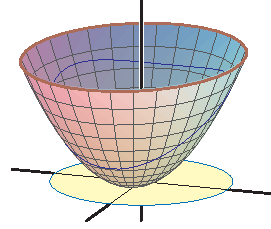
\includegraphics[height=150pt]{images/HW08_1}}
    \put(47,-4){$x$}   \put(172,23){$y$}   \put(83,143){$z$}
    \put(138,-20){{\color{RoyalBlue}$x^2+y^2=16$}} \put(135,-11){{\color{RoyalBlue}\vector(-1,1){20}}}
    \put(-110,23){$2x^2+3y^2-4x+3$}  \put(-25,35){\vector(1,1){45}}
   \end{picture}}
  \end{minipage}
%%%%%%%%%%%%%%%%%%%%%%%%%%%%%%%%%%%%%%%%%%%%%%%%%%%%%%%%%%%%%%%%%%%%%%%%%%%%%%%%%%%%%%%%%%%%%%%%%%%%

%%%%%%%%%%%%%%%%%%%%%%%%%%%%%%%%%%%%%%%%%%%%%%%%%%%%%%%%%%%%%%%%%%%%%%%%%%%%%%%%%%%%%%%%%%%%%%%%%%%%
\item Let $a,b,c$ be positive numbers.
  Use the method of Lagrange multipliers to find the  volume of the largest box in the positive octant  with three faces lying in the
  coordinate planes and one vertex on the plane $x/a+y/b+z/c=1$.    
\vspace{-2pt}
%%%%%%%%%%%%%%%%%%%%%%%%%%%%%%%%%%%%%%%%%%%%%%%%%%%%%%%%%%%%%%%%%%%%%%%%%%%%%%%%%%%%%%%%%%%%%%%%%%%%



%%%%%%%%%%%%%%%%%%%%%%%%%%%%%%%%%%%%%%%%%%%%%%%%%%%%%%%%%%%%%%%%%%%%%%%%%%%%%%%%%%%%%%%%%%%%%%%%%%%%
\item For each of the following, find the maximum of the given function $f(x,y)$ over the bounded set $S$.
  Use the methods of critical point analysis to find the maximum and minimum values over the interior of $S$ and the method
  of Lagrange multipliers to find the maximum and minimum on the boundary of $S$.

  (a) $f(x,y)=x+y-xy$.
  \qquad  $S=\{(x,y)\mid x^2+y^2\leq 9\}$.


  (b) $f(x,y)=1+\frac{x}{1+y^2}$.
      \qquad $S=\{ (x,y) \mid x^2/4 + y^2/9 \leq 1\}$.
\vspace{-2pt}
%%%%%%%%%%%%%%%%%%%%%%%%%%%%%%%%%%%%%%%%%%%%%%%%%%%%%%%%%%%%%%%%%%%%%%%%%%%%%%%%%%%%%%%%%%%%%%%%%%%%


%%%%%%%%%%%%%%%%%%%%%%%%%%%%%%%%%%%%%%%%%%%%%%%%%%%%%%%%%%%%%%%%%%%%%%%%%%%%%%%%%%%%%%%%%%%%%%%%%%%%
\item  Let $w=x_1x_2\dotsb x_n$.
  \begin{enumerate}
  \item Use Lagrange multipliers to maximize $w$ subject to $x_1+x_2+\dotsb+x_n=a$, where $a$ is a fixed positive number and the $x_i$ are
    positive, $x_1,\dotsc,x_n>0$.

  \item Use this to deduce the {\sl\color{Blue}Arithmetic Mean--Geometric Mean Inequality} for positive numbers $a_1,\dotsc,a_n$, which is
    \[
    \sqrt[n]{a_1 a_2 \dotsb a_n}\ \leq\ \frac{a_1+a_2+ \dotsb+a_n}{n}\ .
    \]
  \end{enumerate}
\vspace{-2pt}
%%%%%%%%%%%%%%%%%%%%%%%%%%%%%%%%%%%%%%%%%%%%%%%%%%%%%%%%%%%%%%%%%%%%%%%%%%%%%%%%%%%%%%%%%%%%%%%%%%%%

\end{enumerate}



\end{document}
%%%%%%%%%%%%%%%%%%%%%%%%%%%%%%%%%%%%%%%%%%%%%%%%%%%%%%%%%%%%%%%%%%%
